\subsection{GPU Accelerating \textit{k}mer Counting}
While different GPU accelerated \textit{k}mer counting solutions such as Gerbil \cite{gerbil} have been developed in previous work, we opted to develop our own \textit{k}mer counting method because the \textit{k}mer counting problem solved in KAGE is slightly different than the typical \textit{k}mer counting problem described in section \ref{background:kmers_and_the_kmer_counting_problem}.
Rather than counting the frequency of every observed \textit{k}mer in the input reads, or even the frequency of every observed \textit{k}mer where the frequency is larger than some threshold, KAGE is only interested in counting the observed frequencies for a predetermined set of \textit{k}mers.
This revised problem is easier to solve in practice because the memory constraints are significantly less.
In the interest of brevity, we will refer to the typical \textit{k}mer counting problem described section \ref{background:kmers_and_the_kmer_counting_problem} as \textit{full kmer counting}, and the simpler problem where we only count the frequencies of a predetermined set of \textit{k}mers as \textit{partial kmer counting} \ref{methods:gpu_accelerating_kmer_counting:partial_kmer_counting}.

\definecolor{kmer1}{RGB}{40,40,215}
\definecolor{kmer2}{RGB}{0,150,0}
\definecolor{kmer3}{RGB}{225,30,30}
\definecolor{kmer4}{RGB}{20,150,150}

\begin{figure}[H]
\begin{center}
\scalebox{1}{
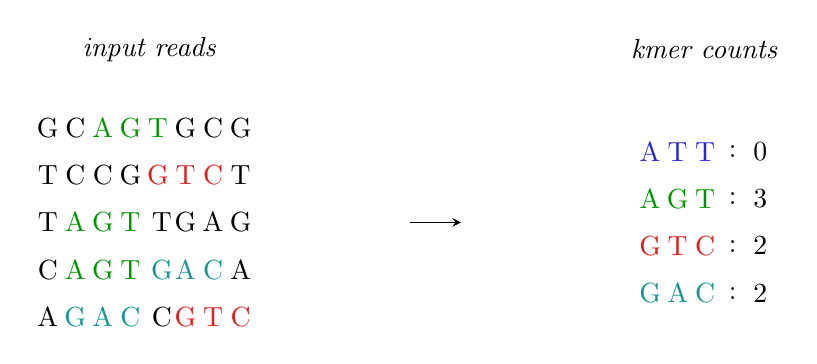
\begin{tikzpicture}
  % titles
  \node at(-0.55,3)(){\textit{input reads}};
  % read 1
  \node at(-1.85,2){G};
  \node at(-1.5,2){C};
  \node at(-1.15,2){\textcolor{kmer2}{A}};
  \node at(-.8,2){\textcolor{kmer2}{G}};
  \node at(-.45,2){\textcolor{kmer2}{T}};
  \node at(-.1,2){G};
  \node at(.25,2){C};
  \node at(.6,2){G};
  % read 2 
  \node at(-1.85,1.4){T};
  \node at(-1.5,1.4){C};
  \node at(-1.15,1.4){C};
  \node at(-.8,1.4){G};
  \node at(-.45,1.4){\textcolor{kmer3}{G}};
  \node at(-.1,1.4){\textcolor{kmer3}{T}};
  \node at(.25,1.4){\textcolor{kmer3}{C}};
  \node at(.6,1.4){T};
  % read 3 
  \node at(-1.85,.8){T};
  \node at(-1.5,.8){\textcolor{kmer2}{A}};
  \node at(-1.15,.8){\textcolor{kmer2}{G}};
  \node at(-.8,.8){\textcolor{kmer2}{T}};
  \node at(-.4,.8){T};
  \node at(-.1,.8){G};
  \node at(.25,.8){A};
  \node at(.6,.8){G};
  % read 4 
  \node at(-1.85,.2){C};
  \node at(-1.5,.2){\textcolor{kmer2}{A}};
  \node at(-1.15,.2){\textcolor{kmer2}{G}};
  \node at(-.8,.2){\textcolor{kmer2}{T}};
  \node at(-.4,.2){\textcolor{kmer4}{G}};
  \node at(-.1,.2){\textcolor{kmer4}{A}};
  \node at(.25,.2){\textcolor{kmer4}{C}};
  \node at(.6,.2){A};
  % read 5 
  \node at(-1.85,-.4){A};
  \node at(-1.5,-.4){\textcolor{kmer4}{G}};
  \node at(-1.15,-.4){\textcolor{kmer4}{A}};
  \node at(-.8,-.4){\textcolor{kmer4}{C}};
  \node at(-.4,-.4){C};
  \node at(-.1,-.4){\textcolor{kmer3}{G}};
  \node at(.25,-.4){\textcolor{kmer3}{T}};
  \node at(.6,-.4){\textcolor{kmer3}{C}};
  % Arrow
  \draw [-stealth](2.75,.8) -- (3.4,.8);
  % k-mer counts
  \node at(6.5,3)(){\textit{kmer counts}};
  % k-mer 1
  \node at(5.8,1.7){\textcolor{kmer1}{A}};
  \node at(6.15,1.7){\textcolor{kmer1}{T}};
  \node at(6.5,1.7){\textcolor{kmer1}{T}};
  \node at(6.85,1.7){:};
  \node at(7.2,1.7){0};
  % k-mer 2 
  \node at(5.8,1.1){\textcolor{kmer2}{A}};
  \node at(6.15,1.1){\textcolor{kmer2}{G}};
  \node at(6.5,1.1){\textcolor{kmer2}{T}};
  \node at(6.85,1.1){:};
  \node at(7.2,1.1){3};
  % k-mer 3 
  \node at(5.8,.5){\textcolor{kmer3}{G}};
  \node at(6.15,.5){\textcolor{kmer3}{T}};
  \node at(6.5,.5){\textcolor{kmer3}{C}};
  \node at(6.85,.5){:};
  \node at(7.2,.5){2};
  % k-mer 4 
  \node at(5.8,-.1){\textcolor{kmer4}{G}};
  \node at(6.15,-.1){\textcolor{kmer4}{A}};
  \node at(6.5,-.1){\textcolor{kmer4}{C}};
  \node at(6.85,-.1){:};
  \node at(7.2,-.1){2};
\end{tikzpicture}
}
\caption{
  In KAGE, we are only interested in counting the observed frequencies of a predefined set of \textit{k}mers, as opposed to every observed \textit{k}mer in the sequenced reads.
}
\label{methods:gpu_accelerating_kmer_counting:partial_kmer_counting}
\end{center}
\end{figure}

\subsubsection{Hash Table Counter based on CuPy}
The Python package npstructures \cite{npstructures} contained a counter object designed to count a static set of \textit{k}mer's frequencies.
This counter object was written in NumPy and implemented a hash table that effectively utilized NumPy's fast array operations to count \textit{k}mers in chunks.
The underlying hash table was based on npstructure's ragged array implementation, which is an effective, NumPy based, two-dimensional array structure where the column lengths can vary.
The array column lengths (bucket sizes) were determined during initialization based on how many of the \textit{k}mers from the unique \textit{k}mer set hashed to that particular bucket.
Because this counter object was implemented using NumPy's array functionality, it served as a good candidate for GPU acceleration where NumPy's CPU vectorization could potentially be manyfold improved by the massively parallel GPU.

In order to GPU accelerate npstructure's counter object we utilized the fact that CuPy's interface is remarkably similar (by design) to that of NumPy.
In fact, CuPy could be described as a GPU accelerated subset of NumPy.
This, in addition to the fact that npstructure's counter object was implemented almost entirely using NumPy, allowed for swift GPU acceleration in a way where we hardly had to write any new code and without having to leave Python at all.

\dirtree{%
  1./.
  2.bin.
}

(explain how to replace numpy with cupy)
\begin{center}
mypackage.my\_funcs.py
\end{center}
\begin{lstlisting}[language=Python,style=pycode]
import numpy as np

def some_func_using_numpy():
  return np.zeros(1000)
\end{lstlisting}

\begin{center}
mypackage.my\_classes.py
\end{center}
\begin{lstlisting}[language=Python,style=pycode]
import numpy as np

class SomeClassUsingNumPy:
  def __init__(self):
    self.data = np.zeros(1000)

  def get_data(self):
    return self.data
\end{lstlisting}

\begin{center}
mypackage.\_\_init\_\_.py
\end{center}
\begin{lstlisting}[language=Python,style=pycode]
from my_funcs import some_func_using_numpy
from my_classes import SomeClassUsingNumPy 

# Swaps NumPy with lib (presumably CuPy)
def set_backend(lib):
  from . import my_funcs
  my_funcs.np = lib

  from . import my_classes
  my_classes.np = lib
\end{lstlisting}

\begin{center}
program.py
\end{center}
\begin{lstlisting}[language=Python,style=pycode]
import cupy as cp

import mypackage
mypackage.set_backend(cp)

array = mypackage.some_func_using_numpy()
type(array) # cupy.ndarray
\end{lstlisting}


\subsubsection{Parallel GPU Hash Table implemented in native CUDA}
...

\subsubsection{Parallel GPU Hash Table without C++}
...

\subsection{GPU Accelerating \textit{k}mer Hashing}


%While one previously developed \textit{k}mer counting tool, Gerbil, supports GPU accelerated \textit{k}mer counting, this tool is designed to solve the full \textit{k}mer counting problem.
%It is not straight-forward to repurpose Gerbil to work with the KAGE genotyping pipeline, for example by first solving the full \textit{k}mer counting problem and then filtering out only the relevant \textit{k}mers.
%This is because Gerbil relies on slow disk operations to store temporary results, and more than that, simply solved a more demanding problem.
%Thus, we decided on implementing our own GPU accelerated \textit{k}mer counting solution. 

%To solve the partial \textit{k}mer counting problem, we implemented a GPU accelerated parallel static hash table to store unique \textit{k}mers as keys and their respective counts as associated values.
